\documentclass[hyperref={pdfpagelabels=false}]{beamer}
\let\Tiny=\tiny
\usepackage{amsmath,amsfonts,amsthm,amssymb}
\usepackage{booktabs}
\usepackage{subfigure}
\usepackage{color}
\usepackage{movie15}
\usepackage{eulervm}
\usepackage{palatino}
%\usepackage{concrete}
%\usepackage{charter}
%\usepackage{courier}
% \usetheme{Warsaw}
% \usefonttheme{serif}
\usetheme{Singapore}

\title{Model Based Control using Lyapunov Stability}
\author{Thomas Denewiler}
%\institute{UCSD/SPAWAR}
\institute{SPAWAR}
%\date{September 21, 2010}

\begin{document}

\begin{frame}
\titlepage
\end{frame}

\begin{frame}{Outline}
\begin{itemize}
\item Types of control laws that can be used.
\item PID controllers.
\item Lyapunov stability theory.
\item Variables used in robot kinematics.
\item Robot kinematic equations.
\item Control Lyapunov function.
\item Resulting control law.
\item Effect of gains on curvature of trajectory.
\item Sample results from a real system.
\item Comparison of PID and model based controllers.
\end{itemize}
\end{frame}

\begin{frame}{Types of Controllers}
\begin{itemize}
\item PID.
\item Fuzzy logic.
\item Model based.
\begin{itemize}
\item LQG - requires linear(ized) system.
\item Lyapunov.
\item Optimal control - minimize/maximize cost/value functions.
\end{itemize}
\end{itemize}
\end{frame}

\begin{frame}[allowframebreaks]{PID Control}
\begin{itemize}
\item Knowledge of system dynamics helpful but not required.
\item Based on error between current and desired state.
\begin{align*}
E_P &= \psi_{\text{ref}_k} - \psi_k \\
E_I &= \sum_{i=0}^{k}E_{P_i}*\Delta_T \\
E_D &= \frac{\psi_k - \psi_{k-1}}{\Delta_T} \\
u &= K_P*E_P + K_I*E_I + K_D*E_D
\end{align*}
\item Gains are tuned to achieve stability of output.

\begin{table}[ht!]
\tiny
\centering
\begin{tabular}{@{}llllr@{}} \toprule
Parameter    & Rise Time      & Overshoot & Settling Time & Steady State Error \\ \midrule
$K_p$        & Decrease       & Increase  & Small Change  & Decrease \\
$K_i$        & Decrease       & Increase  & Increase      & Eliminate \\
$K_d$        & Small Decrease & Decrease  & Decrease      & None \\ \bottomrule
\end{tabular}
\end{table}

\begin{figure}[ht!]
	\centering
	\includegraphics[width=.7\textwidth]{images/pid}
\end{figure}

\item Separate set of gains have to be tuned for different desired velocities.
\item If robot characteristics change all new gains must be developed.
\item Very time consuming.
\end{itemize}
\end{frame}

\begin{frame}{Lyapunov Stability Theory}
\begin{itemize}
\item Need to find a function with the following properties:
\begin{align*}
V(0) &= 0 \\
V(x) &> 0 \in D-\{0\} \\
\dot{V}(x) &< 0 \in D-\{0\}
\end{align*}
\item If $V(x)$ is found then system stability is guaranteed for continuous systems and typically works for sampled systems.
\item Treat errors as "energy" of system and minimize "energy".
\item "Energy" is monotonically decreasing so errors are monotonically decreasing.
\item Trick is to find $V(x)$ containing errors with those properties. Can be very difficult.
\end{itemize}
\end{frame}

\begin{frame}{Valid Control Lyapunov Functions}
\begin{itemize}
\item Valid and invalid functions for $V>0$, $\dot{V}<0$:
\begin{figure}[ht!]
    \centering
    \begin{tabular}{c c}
    \includegraphics[width=.45\textwidth]{images/Vstable} &
    \includegraphics[width=.45\textwidth]{images/Vunstable}
    \end{tabular}
\end{figure}
\end{itemize}
\end{frame}

\begin{frame}{Robot Kinematics - Errors}
\begin{itemize}
\item Errors:
\begin{itemize}
\item $e$, magnitude of translation error vector as measured between current position and goal position,
\item $\theta$, angle between desired heading and translational error vector $e$,
\item $\alpha$, angle between current heading and translational error vector $e$.
\end{itemize}

\begin{figure}[ht!]
	\centering
	\includegraphics[width=.75\textwidth]{images/packbotlyapunov}
\end{figure}

\end{itemize}
\end{frame}

\begin{frame}{Robot Kinematics - Variables}
\begin{itemize}
\item $dx$ and $dy$ are $x$ and $y$ components of $e$.
\item $\psi$ is current heading of robot, get from Kalman filter.
\item $\theta^\star$ is the desired heading of the robot at waypoint which can be:
\begin{itemize}
\item $\theta^\star=0$ is North,
\item $\theta^\star=\pi$ is South,
\item $\theta^\star=\alpha$ would go straight to waypoint,
\item obtained as part of waypoint from MOCU,
\item angle from current waypoint to next waypoint.
\end{itemize}
\item $\phi=\theta^\star-\psi$ is the error between current heading and desired heading.
\end{itemize}
\end{frame}

\begin{frame}{Robot Kinematics - Calculating Errors}
\begin{itemize}
\item Several ways to calculate $e$:
\begin{itemize}
\item $e=\sqrt{dx^2+dy^2}$,
\item use path planner to put carrot out along path to avoid stopping at intermediate waypoints,
\item use maximum of first two methods.
\end{itemize}
\item $\alpha=\tan^{-1}\left(\tfrac{dy}{dx}\right) - \psi$.
\item $\theta=\alpha+\phi$.
\end{itemize}
\end{frame}

\begin{frame}[allowframebreaks]{Robot Kinematics - Equations}
\begin{itemize}
\item Kinematic model describes how robot moves without considering mass, friction or wheels/tracks slipping, etc.
\begin{align}
\label{eq:lyapunovkinematics1}
\begin{split}
\dot{x} &= u\cos(\phi) \\
\dot{y} &= u\sin(\phi) \\
\dot{\phi} &= \omega
\end{split}
\end{align}
\item Convert to polar coordinates:
\begin{align}
\label{eq:lyapunovPolar}
\begin{split}
e &= \sqrt{x^2+y^2} \\
\theta &= \text{atanh}(\tfrac{y}{x}) \\
\alpha &= \theta - \phi
\end{split}
\end{align}
\item Combine (\ref{eq:lyapunovkinematics1}) with (\ref{eq:lyapunovPolar}):
\begin{align*}
\begin{split}
\dot{e} &= -u*\cos(\theta-\phi) \\
\dot{\theta} &= u\frac{\sin\alpha}{e} \\
\dot{\phi} &= \omega
\end{split}
\end{align*}
\item Substitute $\alpha=\theta-\phi$:
\begin{align}
\label{eq:lyapunovkinematics}
\begin{split}
\dot{e} &= -u\cos\alpha \\
\dot{\alpha} &= -\omega + u\frac{\sin\alpha}{e} \\
\dot{\theta} &= u\frac{\sin\alpha}{e}
\end{split}
\end{align}
\end{itemize}
\end{frame}

\begin{frame}{Control Lyapunov Function}
\begin{itemize}
\item Need $V>0$ and $\dot{V}<0$ with $V$ containing $e$, $\alpha$ and $\theta$.
\item $\dot{e}$, $\dot{\alpha}$ and $\dot{\theta}$ from kinematics in (\ref{eq:lyapunovkinematics}).
\begin{align*}
V &= V_1 + V_2 = \frac{1}{2}\lambda e^2 + \frac{1}{2}\left(\alpha^2+h\theta^2\right), \qquad \lambda,h>0 \\
\dot{V}_1 &= \lambda e\dot{e} = \lambda e (-u\cos\alpha) = -\lambda eu\cos\alpha \\
\dot{V}_2 &= \alpha\dot{\alpha}+h\theta\dot{\theta} \\
&= -\alpha\omega + \alpha u\frac{\sin\alpha}{e} + h\theta u\frac{\sin\alpha}{e} \\
&= \alpha\left(-\omega + u\frac{\sin\alpha}{e} + h\theta u\frac{1}{\alpha}\frac{\sin\alpha}{e}\right) \\
&= \alpha\left(-\omega + u\frac{\sin\alpha}{\alpha}\frac{(\alpha+h\theta)}{e}\right)
\end{align*}
\end{itemize}
\end{frame}

\begin{frame}{Control Lyapunov Function - $\dot{V}_1$}
\begin{itemize}
\item $\dot{V}_1<0$ if:
\begin{align*}
u &= \gamma e\cos\alpha, \qquad \gamma>0 \\
\Rightarrow \dot{V}_1 &= -\lambda eu\cos\alpha = -\lambda\gamma e^2\cos^2\alpha \leq 0 \\
\Rightarrow \dot{V}_2 &= \alpha\left(-\omega+u\frac{\sin\alpha}{\alpha}\frac{(\alpha+h\theta)}{e}\right) \\
&= \alpha\left(-\omega+\gamma e\frac{\cos\alpha\sin\alpha}{\alpha}\frac{(\alpha+h\theta)}{e}\right) \\
&= \alpha\left(-\omega+\gamma(\alpha+h\theta)\frac{\cos\alpha\sin\alpha}{\alpha}\right)
\end{align*}
\end{itemize}
\end{frame}

\begin{frame}{Control Lyapunov Function - $\dot{V}_2$}
\begin{itemize}
\item $\dot{V}_2<0$ if:
\begin{align*}
\omega &= k\alpha + \gamma\frac{\cos\alpha\sin\alpha}{\alpha}\left(\alpha+h\theta\right), \qquad k>0 \\
\Rightarrow \dot{V}_2 &= \alpha\left(-k\alpha-\gamma\frac{\cos\alpha\sin\alpha}{\alpha}(\alpha+h\theta)\right. \\
&\qquad + \left.\gamma\frac{\cos\alpha\sin\alpha}{\alpha}(\alpha+h\theta)\right) \\
&= -k\alpha^2 \leq 0
\end{align*}
\end{itemize}
\end{frame}

\begin{frame}{Control Lyapunov Function - Control Law}
\begin{itemize}
\item Combining derivatives yields:
\begin{align*}
\dot{V} = \dot{V}_1 + \dot{V}_2 = -\lambda\gamma e^2\cos^2\alpha - k\alpha^2 \leq 0
\end{align*}
\item $\dot{V}=0$ only when $e=0$ \textit{and} $\alpha=0$ so the system is asymptotically stable meaning that the errors will always be decreasing using this control law.
\begin{align*}
u &= \gamma e\cos\alpha \\
\omega &= k\alpha + \gamma\frac{\cos\alpha\sin\alpha}{\alpha}\left(\alpha+h\theta\right)
\end{align*}
\item $h$, $k$ and $\gamma$ are all positive gains that can be used to tune controller performance.
\end{itemize}
\end{frame}

\begin{frame}{Trajectory Curvature}
\begin{itemize}
\item x
\end{itemize}
\end{frame}

\begin{frame}{Sample Results}
\begin{itemize}
\item Route drawn with MOCU and driven by robot:
\begin{figure}[ht!]
	\centering
    \subfigure{\includegraphics[width=.3\textwidth]{images/20100918_1717_mocu}}
    \quad
	\subfigure{\includegraphics[width=.3\textwidth]{images/20100918_1717_GE_KF}}
\end{figure}
\item Velocities output by model based controller:
\begin{figure}[ht!]
	\centering
	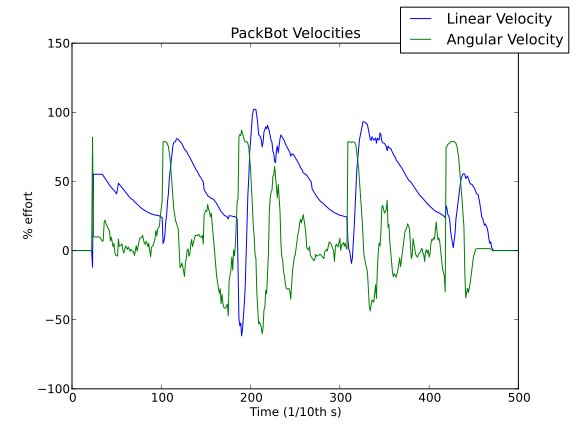
\includegraphics[width=.5\textwidth]{images/20100918_1717_velocities}
\end{figure}
\end{itemize}
\end{frame}

\begin{frame}{Conclusion}
\begin{itemize}
\item Model based controller guarantees stability!
\item Works at multiple linear and angular velocities.
\item Gains modify trajectory curvature, not stability.
\item Handles nonlinear models.
\item Easier to use machine learning with a model compared to PID.
\end{itemize}
\end{frame}

\begin{frame}[allowframebreaks]{References}
\nocite{Khalil02}
\nocite{Rusu05RobotuxLyapunov}
\nocite{Aicardi_UnicycleLyapunov95}
\nocite{Lapierre07}
\nocite{Sights07}
\nocite{ZeiglerNichols42}
\bibliographystyle{plain}
\bibliography{mybib}
\end{frame}

\end{document}
